\problemname {Scholar's Lawn}

Famously at Cambridge, and often copied at other schools, is the tradition of the ``Scholar's Lawn'' -- an area of grass where Fellows of the school, or other distinguished entities, can walk, but regular students cannot.

So, if a student spies a Fellow walking across campus, and wishes to ambush \ldots, er, meet up with them, the student is restricted to walking along a set of narrow paved walkways laid out in various places within the grassy areas, hoping to reach the Fellow's path at the same time or before the Fellow arrives. At the end of the Fellow's path is the Sacred Grove of Academe, off-limits to students, so if the Fellow reaches it before the student, the student is out of luck.

For instance, Figure \ref{fig:paths} shows an area of lawn together with the fixed set of paved walkways (solid lines) and the path taken by a Fellow of the university (dotted line); $F$ and $S$ denote the initial positions of the Fellow and student, respectively. If both travel at the same speed (say, one meter per second), then after $17.67767$ seconds the Fellow will find the student waiting to have a chat at location $(22.5,12.5)$ (marked by the small open circle ``{\Large $\circ$}'').

\begin{figure}[!h]
\centering
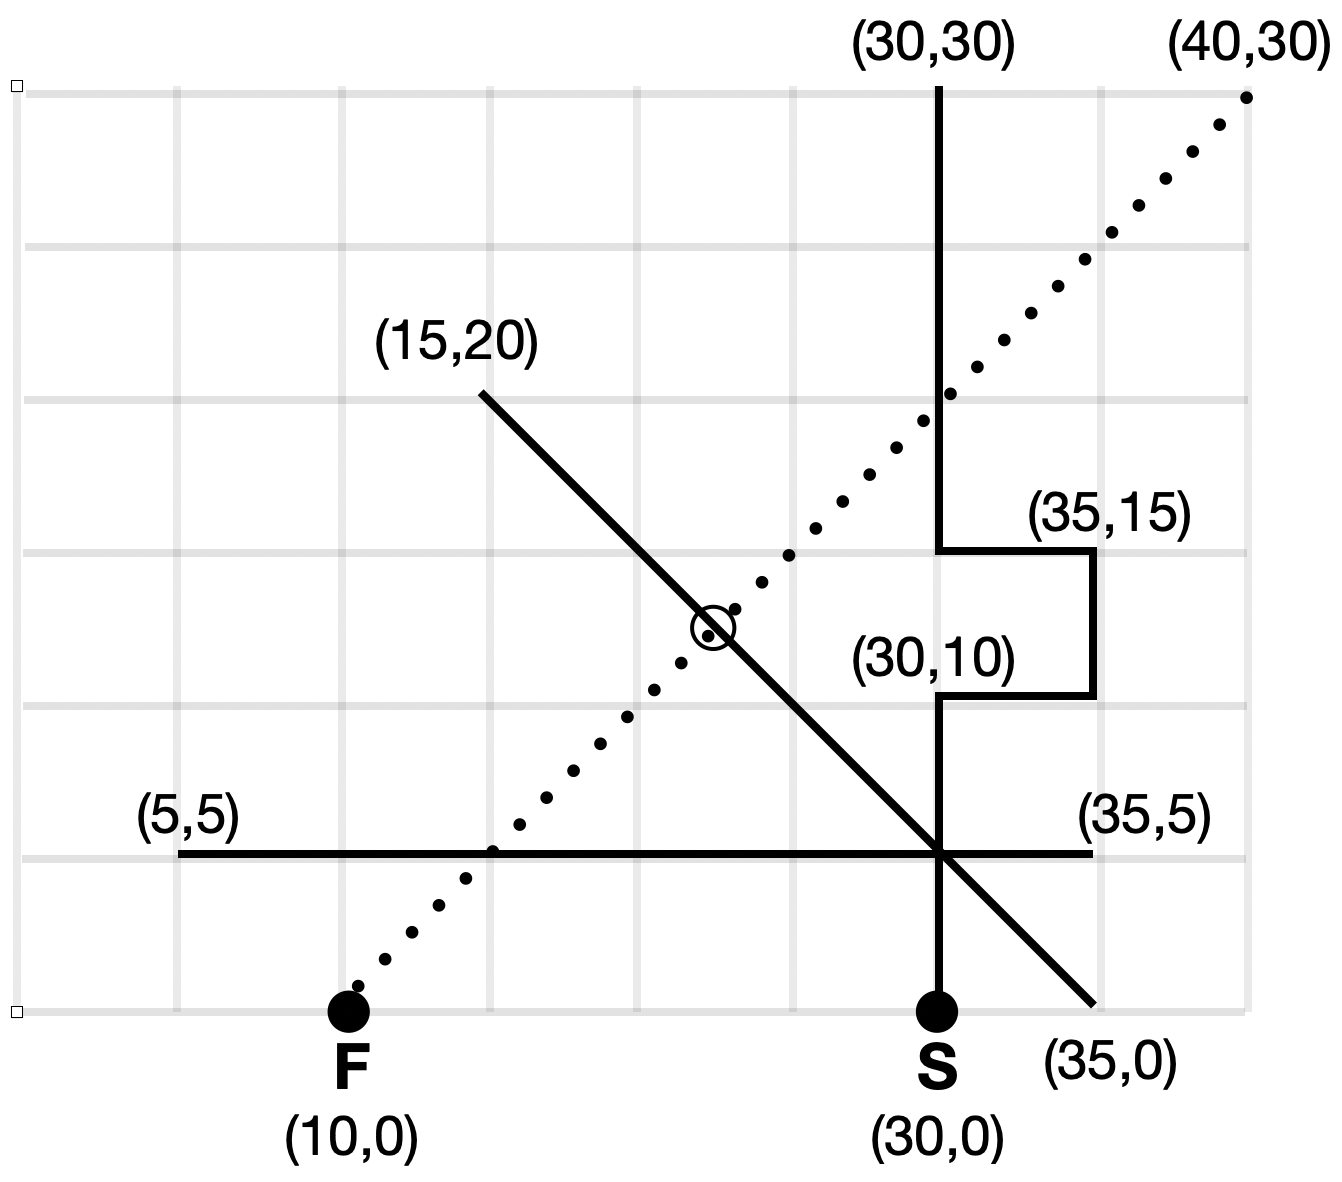
\includegraphics[width=0.5\textwidth]{lawn.png}
\caption{Sample Input 1}
\label{fig:paths}
\end{figure}

\section* {Input}
Input begins with an integer $n$, $1 \le n \le 500$, the number of straight-line walkways. There will then follow $n$ lines, each with $4$ integers, denoting the $(x,y)$ coordinates of the endpoints of each walkway. After that is a line containing three real values $x_s$, $y_s$, $v_s$, where $(x_s,y_s)$ is the position of the student and $v_s$, $0 < v_s \leq 1\,000$, is the student's walking
speed. The point $(x_s,y_s)$ is guaranteed to lie on one of the $n$ paved walkways. The final line contains $5$ numbers. The first $4$ numbers are real numbers $x_{1f}$, $y_{1f}$, $x_{2f}$, $y_{2f}$, $-10\,000 \le x_{1f}, y_{1f},x_{2f},y_{2f} \le 10\,000$, giving the starting position $(x_{1f}, y_{1f})$ of the Fellow and the ending position $(x_{2f}, y_{2f})$ of the Fellow (the last point where the student can reach the Fellow). The final number is a real value $v_f$, $0 < v_f \leq 1\,000$, giving the Fellow's walking speed. All real-valued inputs will have at most four digits after the decimal point.

The Fellow always walks in a straight line.  The student can walk only along walkways, which are assumed to have zero width. If a walkway intersects with another walkway or the Fellow's path, it will do so at a single point. Collinear walkways never intersect one another; similarly, if the Fellow's path and a walkway are collinear, they will not intersect.

\section* {Output}
Output the earliest time $t$ when the student's position and the Fellow's position can coincide at an intersection of a walkway and the Fellow's path. If this is impossible, output the word ``\texttt{Impossible}''. Numeric answers should be
 accurate to within an absolute or relative error of $10^{-6}$.
